\documentclass[aspectratio=169,10pt]{beamer}
\usepackage[T1]{fontenc}
\usepackage[scaled=0.9]{helvet}   % stand-in for Amazon Ember (not installed)
\renewcommand{\familydefault}{\sfdefault}
\usepackage{booktabs,tabularx,multirow,makecell,colortbl,xcolor}
\usepackage{graphicx}
\usepackage{pgfplots}
\pgfplotsset{compat=1.18}
\usepackage{listings}
\usepackage{fontawesome5}

% ---- AWS template palette (dark) ----------------------------------
\definecolor{bgdark}{HTML}{161D26}
\definecolor{panel}{HTML}{232F3E}
\definecolor{awsblue}{HTML}{007DFF}
\definecolor{awspurple}{HTML}{952EFF}
\definecolor{awsmagenta}{HTML}{E433FF}
\definecolor{awsteal}{HTML}{00D6C7}
\definecolor{bodytext}{HTML}{F2F4F7}
\definecolor{inkmuted}{HTML}{A3ACB9}
\definecolor{footc}{HTML}{8B95A3}
\definecolor{rulec}{HTML}{5A6573}
\definecolor{gridc}{HTML}{333E4C}
\definecolor{vendorc}{HTML}{7B8594}
\definecolor{linkc}{HTML}{5FB0FF}
\definecolor{sectag}{HTML}{E433FF}
% extra categorical colours for charts, tuned for the dark background
\definecolor{cat1}{HTML}{EB6834}   % orange
\definecolor{cat2}{HTML}{3B8BEB}   % blue
\definecolor{cat3}{HTML}{1BAF7A}   % aqua

% footer text; override with \renewcommand{\deckfooter}{...} after \documentclass[aspectratio=169,10pt]{beamer}
\usepackage[T1]{fontenc}
\usepackage[scaled=0.9]{helvet}   % stand-in for Amazon Ember (not installed)
\renewcommand{\familydefault}{\sfdefault}
\usepackage{booktabs,tabularx,multirow,makecell,colortbl,xcolor}
\usepackage{graphicx}
\usepackage{pgfplots}
\pgfplotsset{compat=1.18}
\usepackage{listings}
\usepackage{fontawesome5}

% ---- AWS template palette (dark) ----------------------------------
\definecolor{bgdark}{HTML}{161D26}
\definecolor{panel}{HTML}{232F3E}
\definecolor{awsblue}{HTML}{007DFF}
\definecolor{awspurple}{HTML}{952EFF}
\definecolor{awsmagenta}{HTML}{E433FF}
\definecolor{awsteal}{HTML}{00D6C7}
\definecolor{bodytext}{HTML}{F2F4F7}
\definecolor{inkmuted}{HTML}{A3ACB9}
\definecolor{footc}{HTML}{8B95A3}
\definecolor{rulec}{HTML}{5A6573}
\definecolor{gridc}{HTML}{333E4C}
\definecolor{vendorc}{HTML}{7B8594}
\definecolor{linkc}{HTML}{5FB0FF}
\definecolor{sectag}{HTML}{E433FF}
% extra categorical colours for charts, tuned for the dark background
\definecolor{cat1}{HTML}{EB6834}   % orange
\definecolor{cat2}{HTML}{3B8BEB}   % blue
\definecolor{cat3}{HTML}{1BAF7A}   % aqua

% footer text; override with \renewcommand{\deckfooter}{...} after \documentclass[aspectratio=169,10pt]{beamer}
\usepackage[T1]{fontenc}
\usepackage[scaled=0.9]{helvet}   % stand-in for Amazon Ember (not installed)
\renewcommand{\familydefault}{\sfdefault}
\usepackage{booktabs,tabularx,multirow,makecell,colortbl,xcolor}
\usepackage{graphicx}
\usepackage{pgfplots}
\pgfplotsset{compat=1.18}
\usepackage{listings}
\usepackage{fontawesome5}

% ---- AWS template palette (dark) ----------------------------------
\definecolor{bgdark}{HTML}{161D26}
\definecolor{panel}{HTML}{232F3E}
\definecolor{awsblue}{HTML}{007DFF}
\definecolor{awspurple}{HTML}{952EFF}
\definecolor{awsmagenta}{HTML}{E433FF}
\definecolor{awsteal}{HTML}{00D6C7}
\definecolor{bodytext}{HTML}{F2F4F7}
\definecolor{inkmuted}{HTML}{A3ACB9}
\definecolor{footc}{HTML}{8B95A3}
\definecolor{rulec}{HTML}{5A6573}
\definecolor{gridc}{HTML}{333E4C}
\definecolor{vendorc}{HTML}{7B8594}
\definecolor{linkc}{HTML}{5FB0FF}
\definecolor{sectag}{HTML}{E433FF}
% extra categorical colours for charts, tuned for the dark background
\definecolor{cat1}{HTML}{EB6834}   % orange
\definecolor{cat2}{HTML}{3B8BEB}   % blue
\definecolor{cat3}{HTML}{1BAF7A}   % aqua

% footer text; override with \renewcommand{\deckfooter}{...} after \input{preamble}
\newcommand{\deckfooter}{\textcopyright{} \the\year, Amazon Web Services, Inc. or its affiliates.}

% ---- beamer look ---------------------------------------------------
\setbeamercolor{background canvas}{bg=bgdark}
\setbeamercolor{normal text}{fg=bodytext,bg=bgdark}
\setbeamercolor{structure}{fg=awsblue}
\setbeamercolor{frametitle}{fg=white}
\setbeamercolor{itemize item}{fg=awsteal}
\setbeamercolor{itemize subitem}{fg=inkmuted}
\setbeamercolor{enumerate item}{fg=awsteal}
\setbeamercolor{alerted text}{fg=awsmagenta}
\setbeamertemplate{navigation symbols}{}
\setbeamertemplate{itemize items}[square]
\setbeamertemplate{enumerate items}[default]
\setbeamertemplate{caption}[numbered]
\setbeamerfont{itemize/enumerate subbody}{size=\scriptsize}
\setbeamersize{text margin left=8mm,text margin right=8mm}

% section tag shown above each frame title (no divider slides)
\gdef\secname{}
\newcommand{\sect}[1]{\section{#1}\gdef\secname{#1}}
\setbeamertemplate{frametitle}{%
  \nointerlineskip\vskip3.2mm
  \ifx\secname\empty\else{\fontsize{6.5}{7}\selectfont\bfseries\color{sectag}\MakeUppercase{\secname}}\par\vskip0.9mm\fi
  {\fontsize{12.5}{14.5}\selectfont\bfseries\color{white}\insertframetitle}\par\vskip0.6mm}
\setbeamertemplate{headline}{}
\setbeamertemplate{footline}{%
  \hbox to\paperwidth{\hspace*{8mm}{\fontsize{5}{6}\selectfont\color{footc}\deckfooter}\hfill{\fontsize{6}{7}\selectfont\color{footc}\insertframenumber}\hspace*{8mm}}\vskip2.5mm}

% ---- deck macros ---------------------------------------------------
\newcommand{\hl}[1]{\textcolor{awsteal}{\textbf{#1}}}
\newcommand{\src}[1]{\vfill{\tiny\textcolor{footc}{Source: #1}}}
\newcommand{\flabel}[1]{\label{#1}\hypertarget{#1}{}}
% clickable slide references
\newcommand{\sref}[1]{\hyperlink{#1}{\textcolor{linkc}{slide~\pageref*{#1}}}}
\newcommand{\srefs}[2]{\textcolor{linkc}{slides~\hyperlink{#1}{\pageref*{#1}}--\hyperlink{#2}{\pageref*{#2}}}}
\newcommand{\plainen}[1]{\colorbox{panel}{\parbox{\dimexpr\linewidth-2\fboxsep}{\raggedright\footnotesize\textbf{In plain English:} #1}}\par\vspace{1mm}}
\newcommand{\idcard}[1]{\colorbox{panel}{\parbox{\dimexpr\textwidth-2\fboxsep}{\scriptsize #1}}}
\newcommand{\grp}[2]{\multicolumn{#1}{@{}l}{\textcolor{awsteal}{\textit{#2}}}}
\newcommand{\agi}[4]{\hyperlink{#1}{{\large\bfseries\color{awsteal}#2}\quad{\large\bfseries\color{white}#3}}\\[0.5mm]{\small\color{inkmuted}#4}\par\vspace{4mm}}
\newcommand{\bgframe}[1]{\usebackgroundtemplate{\includegraphics[width=\paperwidth,height=\paperheight]{#1}}}

\arrayrulecolor{rulec}
\lstset{basicstyle=\ttfamily\tiny\color{bodytext},breaklines=true,columns=fullflexible,
  backgroundcolor=\color{panel},frame=single,rulecolor=\color{rulec},
  keywordstyle=\color{awsteal}\bfseries,commentstyle=\color{inkmuted},showstringspaces=false}
\renewcommand{\arraystretch}{1.1}
\usetikzlibrary{arrows.meta,positioning,shapes.geometric,calc,fit,backgrounds,shadows,decorations.pathreplacing}
\tikzset{box/.style={draw=awsblue,fill=panel,rounded corners=2pt,align=center,font=\scriptsize,inner sep=3pt,text=bodytext},
         arr/.style={-{Stealth[length=2mm]},thick,awsblue}}
\pgfplotsset{every axis/.append style={axis line style={rulec},tick style={rulec},
  tick label style={text=bodytext},label style={text=bodytext}}}

% numbered table / figure labels (one index across the deck)
\newcounter{tabno}\newcounter{figno}
\newcommand{\tabcap}[1]{\refstepcounter{tabno}{\scriptsize\bfseries\color{awsteal}Table~\thetabno\hspace{0.6em}{\color{bodytext}#1}}\par\vspace{0.2mm}}
\newcommand{\figcap}[1]{\refstepcounter{figno}{\scriptsize\bfseries\color{awsteal}Figure~\thefigno\hspace{0.6em}{\color{bodytext}#1}}\par\vspace{0.2mm}}

% ---- table helpers -------------------------------------------------
\newcommand{\tb}[1]{\texttt{#1}}
\newcolumntype{P}[1]{>{\raggedright\arraybackslash}p{#1}}
\newcolumntype{Y}{>{\raggedright\arraybackslash}X}
% substrate names in their fixed chart colours (blue / orange / aqua)
\newcommand{\smv}{\textcolor{cat2}{\textbf{microVM}}}
\newcommand{\sm}{\textcolor{cat1}{\textbf{m5}}}
\newcommand{\sg}{\textcolor{cat3}{\textbf{g6}}}

\newcommand{\deckfooter}{\textcopyright{} \the\year, Amazon Web Services, Inc. or its affiliates.}

% ---- beamer look ---------------------------------------------------
\setbeamercolor{background canvas}{bg=bgdark}
\setbeamercolor{normal text}{fg=bodytext,bg=bgdark}
\setbeamercolor{structure}{fg=awsblue}
\setbeamercolor{frametitle}{fg=white}
\setbeamercolor{itemize item}{fg=awsteal}
\setbeamercolor{itemize subitem}{fg=inkmuted}
\setbeamercolor{enumerate item}{fg=awsteal}
\setbeamercolor{alerted text}{fg=awsmagenta}
\setbeamertemplate{navigation symbols}{}
\setbeamertemplate{itemize items}[square]
\setbeamertemplate{enumerate items}[default]
\setbeamertemplate{caption}[numbered]
\setbeamerfont{itemize/enumerate subbody}{size=\scriptsize}
\setbeamersize{text margin left=8mm,text margin right=8mm}

% section tag shown above each frame title (no divider slides)
\gdef\secname{}
\newcommand{\sect}[1]{\section{#1}\gdef\secname{#1}}
\setbeamertemplate{frametitle}{%
  \nointerlineskip\vskip3.2mm
  \ifx\secname\empty\else{\fontsize{6.5}{7}\selectfont\bfseries\color{sectag}\MakeUppercase{\secname}}\par\vskip0.9mm\fi
  {\fontsize{12.5}{14.5}\selectfont\bfseries\color{white}\insertframetitle}\par\vskip0.6mm}
\setbeamertemplate{headline}{}
\setbeamertemplate{footline}{%
  \hbox to\paperwidth{\hspace*{8mm}{\fontsize{5}{6}\selectfont\color{footc}\deckfooter}\hfill{\fontsize{6}{7}\selectfont\color{footc}\insertframenumber}\hspace*{8mm}}\vskip2.5mm}

% ---- deck macros ---------------------------------------------------
\newcommand{\hl}[1]{\textcolor{awsteal}{\textbf{#1}}}
\newcommand{\src}[1]{\vfill{\tiny\textcolor{footc}{Source: #1}}}
\newcommand{\flabel}[1]{\label{#1}\hypertarget{#1}{}}
% clickable slide references
\newcommand{\sref}[1]{\hyperlink{#1}{\textcolor{linkc}{slide~\pageref*{#1}}}}
\newcommand{\srefs}[2]{\textcolor{linkc}{slides~\hyperlink{#1}{\pageref*{#1}}--\hyperlink{#2}{\pageref*{#2}}}}
\newcommand{\plainen}[1]{\colorbox{panel}{\parbox{\dimexpr\linewidth-2\fboxsep}{\raggedright\footnotesize\textbf{In plain English:} #1}}\par\vspace{1mm}}
\newcommand{\idcard}[1]{\colorbox{panel}{\parbox{\dimexpr\textwidth-2\fboxsep}{\scriptsize #1}}}
\newcommand{\grp}[2]{\multicolumn{#1}{@{}l}{\textcolor{awsteal}{\textit{#2}}}}
\newcommand{\agi}[4]{\hyperlink{#1}{{\large\bfseries\color{awsteal}#2}\quad{\large\bfseries\color{white}#3}}\\[0.5mm]{\small\color{inkmuted}#4}\par\vspace{4mm}}
\newcommand{\bgframe}[1]{\usebackgroundtemplate{\includegraphics[width=\paperwidth,height=\paperheight]{#1}}}

\arrayrulecolor{rulec}
\lstset{basicstyle=\ttfamily\tiny\color{bodytext},breaklines=true,columns=fullflexible,
  backgroundcolor=\color{panel},frame=single,rulecolor=\color{rulec},
  keywordstyle=\color{awsteal}\bfseries,commentstyle=\color{inkmuted},showstringspaces=false}
\renewcommand{\arraystretch}{1.1}
\usetikzlibrary{arrows.meta,positioning,shapes.geometric,calc,fit,backgrounds,shadows,decorations.pathreplacing}
\tikzset{box/.style={draw=awsblue,fill=panel,rounded corners=2pt,align=center,font=\scriptsize,inner sep=3pt,text=bodytext},
         arr/.style={-{Stealth[length=2mm]},thick,awsblue}}
\pgfplotsset{every axis/.append style={axis line style={rulec},tick style={rulec},
  tick label style={text=bodytext},label style={text=bodytext}}}

% numbered table / figure labels (one index across the deck)
\newcounter{tabno}\newcounter{figno}
\newcommand{\tabcap}[1]{\refstepcounter{tabno}{\scriptsize\bfseries\color{awsteal}Table~\thetabno\hspace{0.6em}{\color{bodytext}#1}}\par\vspace{0.2mm}}
\newcommand{\figcap}[1]{\refstepcounter{figno}{\scriptsize\bfseries\color{awsteal}Figure~\thefigno\hspace{0.6em}{\color{bodytext}#1}}\par\vspace{0.2mm}}

% ---- table helpers -------------------------------------------------
\newcommand{\tb}[1]{\texttt{#1}}
\newcolumntype{P}[1]{>{\raggedright\arraybackslash}p{#1}}
\newcolumntype{Y}{>{\raggedright\arraybackslash}X}
% substrate names in their fixed chart colours (blue / orange / aqua)
\newcommand{\smv}{\textcolor{cat2}{\textbf{microVM}}}
\newcommand{\sm}{\textcolor{cat1}{\textbf{m5}}}
\newcommand{\sg}{\textcolor{cat3}{\textbf{g6}}}

\newcommand{\deckfooter}{\textcopyright{} \the\year, Amazon Web Services, Inc. or its affiliates.}

% ---- beamer look ---------------------------------------------------
\setbeamercolor{background canvas}{bg=bgdark}
\setbeamercolor{normal text}{fg=bodytext,bg=bgdark}
\setbeamercolor{structure}{fg=awsblue}
\setbeamercolor{frametitle}{fg=white}
\setbeamercolor{itemize item}{fg=awsteal}
\setbeamercolor{itemize subitem}{fg=inkmuted}
\setbeamercolor{enumerate item}{fg=awsteal}
\setbeamercolor{alerted text}{fg=awsmagenta}
\setbeamertemplate{navigation symbols}{}
\setbeamertemplate{itemize items}[square]
\setbeamertemplate{enumerate items}[default]
\setbeamertemplate{caption}[numbered]
\setbeamerfont{itemize/enumerate subbody}{size=\scriptsize}
\setbeamersize{text margin left=8mm,text margin right=8mm}

% section tag shown above each frame title (no divider slides)
\gdef\secname{}
\newcommand{\sect}[1]{\section{#1}\gdef\secname{#1}}
\setbeamertemplate{frametitle}{%
  \nointerlineskip\vskip3.2mm
  \ifx\secname\empty\else{\fontsize{6.5}{7}\selectfont\bfseries\color{sectag}\MakeUppercase{\secname}}\par\vskip0.9mm\fi
  {\fontsize{12.5}{14.5}\selectfont\bfseries\color{white}\insertframetitle}\par\vskip0.6mm}
\setbeamertemplate{headline}{}
\setbeamertemplate{footline}{%
  \hbox to\paperwidth{\hspace*{8mm}{\fontsize{5}{6}\selectfont\color{footc}\deckfooter}\hfill{\fontsize{6}{7}\selectfont\color{footc}\insertframenumber}\hspace*{8mm}}\vskip2.5mm}

% ---- deck macros ---------------------------------------------------
\newcommand{\hl}[1]{\textcolor{awsteal}{\textbf{#1}}}
\newcommand{\src}[1]{\vfill{\tiny\textcolor{footc}{Source: #1}}}
\newcommand{\flabel}[1]{\label{#1}\hypertarget{#1}{}}
% clickable slide references
\newcommand{\sref}[1]{\hyperlink{#1}{\textcolor{linkc}{slide~\pageref*{#1}}}}
\newcommand{\srefs}[2]{\textcolor{linkc}{slides~\hyperlink{#1}{\pageref*{#1}}--\hyperlink{#2}{\pageref*{#2}}}}
\newcommand{\plainen}[1]{\colorbox{panel}{\parbox{\dimexpr\linewidth-2\fboxsep}{\raggedright\footnotesize\textbf{In plain English:} #1}}\par\vspace{1mm}}
\newcommand{\idcard}[1]{\colorbox{panel}{\parbox{\dimexpr\textwidth-2\fboxsep}{\scriptsize #1}}}
\newcommand{\grp}[2]{\multicolumn{#1}{@{}l}{\textcolor{awsteal}{\textit{#2}}}}
\newcommand{\agi}[4]{\hyperlink{#1}{{\large\bfseries\color{awsteal}#2}\quad{\large\bfseries\color{white}#3}}\\[0.5mm]{\small\color{inkmuted}#4}\par\vspace{4mm}}
\newcommand{\bgframe}[1]{\usebackgroundtemplate{\includegraphics[width=\paperwidth,height=\paperheight]{#1}}}

\arrayrulecolor{rulec}
\lstset{basicstyle=\ttfamily\tiny\color{bodytext},breaklines=true,columns=fullflexible,
  backgroundcolor=\color{panel},frame=single,rulecolor=\color{rulec},
  keywordstyle=\color{awsteal}\bfseries,commentstyle=\color{inkmuted},showstringspaces=false}
\renewcommand{\arraystretch}{1.1}
\usetikzlibrary{arrows.meta,positioning,shapes.geometric,calc,fit,backgrounds,shadows,decorations.pathreplacing}
\tikzset{box/.style={draw=awsblue,fill=panel,rounded corners=2pt,align=center,font=\scriptsize,inner sep=3pt,text=bodytext},
         arr/.style={-{Stealth[length=2mm]},thick,awsblue}}
\pgfplotsset{every axis/.append style={axis line style={rulec},tick style={rulec},
  tick label style={text=bodytext},label style={text=bodytext}}}

% numbered table / figure labels (one index across the deck)
\newcounter{tabno}\newcounter{figno}
\newcommand{\tabcap}[1]{\refstepcounter{tabno}{\scriptsize\bfseries\color{awsteal}Table~\thetabno\hspace{0.6em}{\color{bodytext}#1}}\par\vspace{0.2mm}}
\newcommand{\figcap}[1]{\refstepcounter{figno}{\scriptsize\bfseries\color{awsteal}Figure~\thefigno\hspace{0.6em}{\color{bodytext}#1}}\par\vspace{0.2mm}}

% ---- table helpers -------------------------------------------------
\newcommand{\tb}[1]{\texttt{#1}}
\newcolumntype{P}[1]{>{\raggedright\arraybackslash}p{#1}}
\newcolumntype{Y}{>{\raggedright\arraybackslash}X}
% substrate names in their fixed chart colours (blue / orange / aqua)
\newcommand{\smv}{\textcolor{cat2}{\textbf{microVM}}}
\newcommand{\sm}{\textcolor{cat1}{\textbf{m5}}}
\newcommand{\sg}{\textcolor{cat3}{\textbf{g6}}}

% First-call deck (17 slides) for technical decision-makers. Every number comes from the deep-dive deck
% (agentic_rl_on_agentcore.tex), which cites its logs; the "Deep dive:" line on each slide names the
% deep-dive slide behind it.
\renewcommand{\deckfooter}{Agentic RL sandboxes on AWS \textperiodcentered{} first call}
\newcommand{\deep}[1]{\par\vspace{0.5mm}{\tiny\textcolor{footc}{Deep dive: #1}}}
\newcommand{\settag}[1]{\gdef\secname{#1}}
% one challenge slide: challenge | what we did | proof
\newcommand{\chal}[3]{\colorbox{panel}{\parbox[t][25mm]{\dimexpr\linewidth-2\fboxsep}{\raggedright\vspace{1.5mm}%
  {\normalsize\bfseries\color{#1}#2}\par\vspace{1.5mm}\small #3}}}

\title{Agentic RL Sandboxes on AWS}
\date{October 2026}

\begin{document}

%====================================================================
{\bgframe{art/bg_title.jpg}
\begin{frame}[plain]
\vspace*{4mm}
\begin{minipage}{0.50\textwidth}\raggedright
{\fontsize{22}{26}\selectfont\bfseries\color{white}Agentic RL Sandboxes on AWS\par}
\vspace{3mm}
{\normalsize\color{white}A sandbox per episode, at RL scale, with Amazon Bedrock AgentCore and EC2\par}
\vspace{8mm}
{\small\color{white}\textbf{Kaige Yang}\\Senior Applied Scientist, AWS\par}
\end{minipage}
\end{frame}}

%====================================================================
\settag{At a glance}
\begin{frame}{At a glance: one agentic-RL stack on AWS, built for the hard cases}
\begin{columns}[T]
\column{0.49\textwidth}
{\normalsize\textbf{\textcolor{awsteal}{Architecture}}}\par\vspace{1mm}
\centering
\begin{tikzpicture}[x=1mm,y=1mm,scale=0.8,transform shape, every node/.style={font=\scriptsize},
  lbl/.style={font=\tiny,text=inkmuted,align=center},
  zone/.style={dashed,rounded corners=3pt,inner sep=1.2mm}]
\node[box,draw=awspurple,text width=20mm,minimum height=26mm] (tr) at (0,0) {\textbf{slime}\\trainer\\[0.5mm]GRPO +\\SGLang\\[0.5mm]\textcolor{awsteal}{\textbf{router}}};
\node[box,draw=cat2,text width=24mm] (mv) at (36,12) {\textcolor{cat2}{\textbf{microVM}}};
\node[box,draw=cat3,text width=24mm] (gi) at (36,4.8) {\textcolor{cat3}{\textbf{GPU Instance}}};
\node[box,draw=cat1,text width=24mm] (m5) at (36,-4.8) {\textcolor{cat1}{\textbf{m5 pool}}};
\node[box,draw=cat1,text width=24mm] (gp) at (36,-12) {\textcolor{cat1}{\textbf{GPU pool}}};
\begin{scope}[on background layer]
\node[zone,draw=cat2,fit=(mv)(gi),label={[lbl]above:AgentCore (managed)}] (ac) {};
\node[zone,draw=cat1,fit=(m5)(gp),label={[lbl]below:plain EC2 (our code)}] (ec) {};
\end{scope}
\draw[arr] ($(tr.east)+(0,5)$) -- (ac.west);
\draw[arr,cat1] ($(tr.east)+(0,-5)$) -- (ec.west);
\end{tikzpicture}
\par\vspace{0.5mm}\raggedright
{\normalsize\textbf{\textcolor{awsteal}{Key contributions}}}
\begin{itemize}\footnotesize\setlength{\itemsep}{0.3mm}
\item \textbf{slime $\times$ AgentCore}: RL sandboxes, slime unpatched.
\item \textbf{Hybrid, every use case}: 2 AgentCore + 2 EC2.
\item \textbf{Pre-open}: sandboxes ready before the episode.
\item \textbf{Decoupled harness}: Claude Code / Codex Runtime.
\item \textbf{Skills}: read with \tb{bash}, removed before grading.
\end{itemize}
\column{0.47\textwidth}
{\normalsize\textbf{\textcolor{awsteal}{Challenges solved}}}
\begin{itemize}\footnotesize\setlength{\itemsep}{0.3mm}
\item \textbf{x86 and arm64}: microVMs are arm64 only; x86-only tasks run on the x86 m5.
\item \textbf{Large images}: over the 2\,GB microVM cap (up to 6.7\,GB) on the m5; the 17\,GB KernelBench image on the EC2 GPU pool.
\item \textbf{Multi-container tasks}: docker compose on the m5, 12 of 12 usable.
\item \textbf{GPU tasks}: \hl{261}/270 KernelBench on AgentCore GPU Instances + an EC2 GPU pool.
\item \textbf{Cold starts}: pre-open sandboxes and instances ahead; median wait \hl{0\,s}, \hl{1{,}188} episodes/h.
\item \textbf{Sticky routing}: one session and one engine per episode, so every turn hits the same sandbox and KV cache.
\item \textbf{Result}: \hl{212}/241 Terminal-Bench usable; \hl{0.34\,\%} infra errors.
\end{itemize}
\end{columns}
\par\vskip 0pt plus 1filll
\deep{``At a glance''}
\end{frame}

%====================================================================
\settag{Concepts}
\begin{frame}{Agentic RL: the model learns by acting in a real machine}
\centering
\begin{tikzpicture}[x=1mm,y=1mm, every node/.style={font=\small},
  lbl/.style={font=\scriptsize,text=inkmuted,align=center},
  num/.style={circle,fill=awsteal,text=bgdark,font=\scriptsize\bfseries,inner sep=0.8pt,minimum size=4.2mm}]
\node[box,text width=26mm,font=\small] (task) at (0,10) {\textbf{Task}\\instruction +\\environment};
\node[box,draw=cat2,text width=40mm,minimum height=20mm,font=\small] (sb) at (46,10) {\textbf{Sandbox}\\the task's own machine;\\the agent runs commands\\hidden tests score the end};
\node[box,draw=awspurple,text width=34mm,font=\small] (inf) at (96,22) {\textbf{Policy}\\the model in training};
\node[box,draw=awspurple,text width=34mm,font=\small] (trn) at (96,-2) {\textbf{Trainer}\\GRPO: compare tries,\\reinforce the better};
\draw[arr] (task) -- node[lbl,above]{open} (sb);
\draw[arr,awsteal] ($(sb.east)+(0,6)$) -- node[lbl,above,sloped]{each turn: next action} (inf.west);
\draw[arr] ($(sb.east)+(0,-6)$) -- node[lbl,below,sloped]{tokens + reward} (trn.west);
\draw[arr,awspurple] (trn) -- node[lbl,right]{new weights} (inf);
\end{tikzpicture}
\par\vspace{3mm}\raggedright
\begin{columns}[T]
\column{0.48\textwidth}
\begin{itemize}\small\setlength{\itemsep}{1mm}
\item \textbf{Every try needs its own clean machine}: the agent installs, edits and breaks things.
\item \textbf{Thousands of tries per hour}: here 1{,}188 episodes/h, 32 at once.
\end{itemize}
\column{0.48\textwidth}
\begin{itemize}\small\setlength{\itemsep}{1mm}
\item \textbf{The score must be honest}: RL optimizes the reward, so any shortcut gets learned.
\item \textbf{The sandbox is the RL environment}: if it's slow, wrong or leaky, training is too.
\end{itemize}
\end{columns}
\par\vskip 0pt plus 1filll
\deep{``Agentic RL workflow''}
\end{frame}

%====================================================================
\begin{frame}{Amazon Bedrock AgentCore Runtime: a managed machine per session}
\begin{columns}[T]
\column{0.50\textwidth}
{\normalsize\textbf{\textcolor{cat2}{microVM}} \small(the default)}
\begin{itemize}\small\setlength{\itemsep}{1mm}
\item One session = one isolated microVM with its own kernel; a new session id = a new machine.
\item Fully managed: boot, isolation, idle reclaim, teardown.
\item Opens in \hl{0.9\,s} (median), from your container image.
\end{itemize}
\vspace{1mm}
{\normalsize\textbf{\textcolor{cat3}{GPU Instance}} \small(capacity provider)}
\begin{itemize}\small\setlength{\itemsep}{1mm}
\item Same API, a whole GPU machine per session (g5/g6e here).
\item Opens in 143\,s: a fresh machine every time.
\end{itemize}
\column{0.46\textwidth}
\tabcap{What it doesn't do, so we add plain EC2}
\small\setlength{\tabcolsep}{3pt}\renewcommand{\arraystretch}{1.3}
\begin{tabularx}{\linewidth}{@{}Y P{0.34\linewidth}@{}}
\toprule
\textbf{Limit} & \textbf{Workaround}\\
\midrule
no Docker daemon, no root capabilities & EC2 \textcolor{cat1}{\textbf{m5}} pool\\
images capped at 2\,GB & EC2 (no cap)\\
microVMs are arm64 only & EC2 x86\\
1 session = 1 machine, no warm reuse on GPU & EC2 \textcolor{cat1}{\textbf{GPU pool}}\\
\bottomrule
\end{tabularx}
\end{columns}
\par\vskip 0pt plus 1filll
\plainen{AgentCore gives every episode its own managed machine in under a second. Where a task needs Docker, root, a big image or warm GPUs, we fill the gap with plain EC2 behind the same API.}
\deep{``AgentCore Runtime foundations'', ``What AgentCore can't do''}
\end{frame}

%====================================================================
\settag{The problem}
\begin{frame}{The workload: 511 real agentic tasks, two very different kinds}
\begin{columns}[T]
\column{0.48\textwidth}
\colorbox{panel}{\parbox[t][44mm]{\dimexpr\linewidth-2\fboxsep}{\raggedright\vspace{1.5mm}
{\large\bfseries\textcolor{awsteal}{Terminal-Bench}} {\small 241 tasks}\par\vspace{1mm}
\small Fix or build something in a Linux machine, with shell commands.\par\vspace{2mm}
\textbf{Example} \tb{postgres-csv-clean}: ``clean the customer data in PostgreSQL, export \tb{cleaned\_customers.csv}''.\par\vspace{2mm}
\textbf{Machine}: an app container + a Postgres sidecar.\par\vspace{1mm}
\textbf{Scored}: hidden tests check the CSV and that the work ran in Postgres.}}
\column{0.48\textwidth}
\colorbox{panel}{\parbox[t][44mm]{\dimexpr\linewidth-2\fboxsep}{\raggedright\vspace{1.5mm}
{\large\bfseries\textcolor{awsteal}{KernelBench}} {\small 270 tasks}\par\vspace{1mm}
\small Rewrite a PyTorch model as a faster GPU kernel.\par\vspace{2mm}
\textbf{Example}: ``here is \tb{Model}; write \tb{ModelNew}: same output, on the GPU, faster''.\par\vspace{2mm}
\textbf{Machine}: a GPU with CUDA PyTorch.\par\vspace{1mm}
\textbf{Scored}: a hidden checker compares outputs and times both: full reward only if $\ge$1.10$\times$ faster.}}
\end{columns}
\par\vskip 0pt plus 1filll
\plainen{every task is a small broken computer plus a hidden exam. Each needs its own image, some need several containers, root or a GPU.}
\deep{``The agentic tasks in this solution'', ``One example from each dataset''}
\end{frame}

%====================================================================
\begin{frame}{16 challenges every agentic-RL sandbox must solve, in four groups}
\begin{columns}[T]
\column{0.48\textwidth}
\chal{awsteal}{1 \quad Every task gets its environment}{one image per task (241 Dockerfiles) $\cdot$ images up to 6.7\,GB vs a 2\,GB cap $\cdot$ x86-only tasks on arm64 $\cdot$ multi-container tasks $\cdot$ root and capabilities $\cdot$ GPUs}
\par\vspace{2mm}
\chal{awsteal}{3 \quad Rewards you can trust}{no leaks between episodes $\cdot$ hidden tests the agent can't read or game $\cdot$ tasks whose own solution fails $\cdot$ all-or-nothing scores give GRPO no signal}
\column{0.48\textwidth}
\chal{awsteal}{2 \quad The trainer never waits}{cold starts of 1\,s to 2.5\,min vs a $\sim$11\,s agent loop $\cdot$ idle sessions reclaimed after 15\,min $\cdot$ concurrency and quotas $\cdot$ long or hung tool calls}
\par\vspace{2mm}
\chal{awsteal}{4 \quad Safe, reliable, affordable}{the agent runs untrusted code yet must reach the trainer, with no public ports $\cdot$ nothing left running after a crash $\cdot$ GPU machines dominate the bill}
\end{columns}
\par\vskip 0pt plus 1filll
\plainen{the next four slides take one group each: the challenge, what we did, and the number that shows it works.}
\deep{``16 challenges every agentic-RL sandbox must solve''}
\end{frame}

%====================================================================
\settag{Our solution}
\begin{frame}{The solution: one RL loop, four sandbox substrates, chosen per task}
\centering
\begin{tikzpicture}[x=1mm,y=1mm, every node/.style={font=\small},
  lbl/.style={font=\scriptsize,text=inkmuted,align=center},
  zone/.style={dashed,rounded corners=3pt,inner sep=2mm}]
\node[box,draw=awspurple,text width=34mm,minimum height=26mm,font=\small] (tr) at (0,10) {\textbf{slime trainer}\\(open-source RL)\\[1mm]GRPO training\\+ SGLang inference\\[1mm]\textcolor{awsteal}{\textbf{our router}}: task $\rightarrow$\\its substrate};
\node[box,draw=cat2,text width=40mm] (mv) at (68,26) {\textbf{\textcolor{cat2}{AgentCore microVM}}\\Terminal-Bench, 162 tasks};
\node[box,draw=cat3,text width=40mm] (gi) at (68,15) {\textbf{\textcolor{cat3}{AgentCore GPU Instance}}\\KernelBench level 1};
\node[box,draw=cat1,text width=40mm] (m5) at (68,2) {\textbf{\textcolor{cat1}{EC2 m5 pool}}\\Terminal-Bench, 50 tasks\\(Docker, root, x86, big images)};
\node[box,draw=cat1,text width=40mm] (gp) at (68,-10) {\textbf{\textcolor{cat1}{EC2 GPU pool}}\\KernelBench levels 2--4};
\begin{scope}[on background layer]
\node[zone,draw=cat2,fit=(mv)(gi),label={[lbl,anchor=west]east:\textbf{managed by AgentCore}}] (ac) {};
\node[zone,draw=cat1,fit=(m5)(gp),label={[lbl,anchor=west]east:\textbf{managed by our code}}] (ec) {};
\end{scope}
\draw[arr] ($(tr.east)+(0,6)$) -- node[lbl,above,sloped]{InvokeAgentRuntime} (ac.west);
\draw[arr,cat1] ($(tr.east)+(0,-6)$) -- node[lbl,below,sloped]{EC2 API + HTTP} (ec.west);
\end{tikzpicture}
\par\vspace{2mm}\raggedright
\begin{columns}[T]
\column{0.32\textwidth}
\small\textbf{One code path}: harness, grader and reward never know the substrate.
\column{0.32\textwidth}
\small\textbf{Routing is data}: each task goes where its own reference solution passes.
\column{0.32\textwidth}
\small\textbf{slime unpatched}: we plug in through its extension points.
\end{columns}
\par\vskip 0pt plus 1filll
\deep{``The architecture'', ``Why four substrates''}
\end{frame}

%====================================================================
\begin{frame}{Why a hybrid: each substrate covers what the others can't}
\begin{columns}[T]
\column{0.24\textwidth}
\colorbox{panel}{\parbox[t][38mm]{\dimexpr\linewidth-2\fboxsep}{\raggedright\vspace{1mm}\scriptsize
{\footnotesize\bfseries\textcolor{cat2}{AgentCore microVM}}\par
{\tiny\textcolor{inkmuted}{Terminal-Bench, 162 tasks}}\par\vspace{1mm}
\textbf{Why}: fully managed, own kernel per session, \hl{0.9\,s} to open.\par\vspace{1mm}
\textbf{Can't}: arm64 only; 2\,GB image cap; no Docker or root; no GPU.}}
\column{0.24\textwidth}
\colorbox{panel}{\parbox[t][38mm]{\dimexpr\linewidth-2\fboxsep}{\raggedright\vspace{1mm}\scriptsize
{\footnotesize\bfseries\textcolor{cat1}{EC2 m5 pool}}\par
{\tiny\textcolor{inkmuted}{Terminal-Bench, 50 tasks}}\par\vspace{1mm}
\textbf{Why}: a whole VM with Docker, as Terminal-Bench runs upstream: x86, any image size, root, sidecars.\par\vspace{1mm}
\textbf{Why not AgentCore}: a CPU Instance has the same limits as a microVM.\par\vspace{1mm}
\textbf{Price}: we own launch, reset and clean-up.}}
\column{0.24\textwidth}
\colorbox{panel}{\parbox[t][38mm]{\dimexpr\linewidth-2\fboxsep}{\raggedright\vspace{1mm}\scriptsize
{\footnotesize\bfseries\textcolor{cat3}{AgentCore GPU Instance}}\par
{\tiny\textcolor{inkmuted}{KernelBench level 1, 95 tasks}}\par\vspace{1mm}
\textbf{Why}: a small image that needs only a GPU; same API as a microVM, managed, a fresh machine per session.\par\vspace{1mm}
\textbf{Can't}: microVMs have no GPU; \textbf{143\,s} to open, as CUDA torch can't fit the 2\,GB cap.}}
\column{0.24\textwidth}
\colorbox{panel}{\parbox[t][38mm]{\dimexpr\linewidth-2\fboxsep}{\raggedright\vspace{1mm}\scriptsize
{\footnotesize\bfseries\textcolor{cat1}{EC2 GPU pool}}\par
{\tiny\textcolor{inkmuted}{KernelBench levels 2--4, 166 tasks}}\par\vspace{1mm}
\textbf{Why}: torch baked in, warm GPUs, a fresh container per episode: \hl{1.4\,s} to open.\par\vspace{1mm}
\textbf{Why not AgentCore}: level 4 needs a 17\,GB image; 166 tasks at 143\,s each.\par\vspace{1mm}
\textbf{Price}: we own the lifecycle and verified reset.}}
\end{columns}
\par\vspace{2mm}
{\small\textbf{Without the hybrid}: microVMs alone cover 162 of 241 Terminal-Bench tasks and none of KernelBench. With all four: \hl{212} and \hl{261} of 270, behind one API, in one training batch.\par}
\par\vskip 0pt plus 1filll
\plainen{use AgentCore wherever a task fits its contract; use plain EC2 when a task needs a whole machine with Docker and root, or a big image with a fast GPU open. The router decides per task, by measurement.}
\deep{``Why four substrates'', ``What AgentCore can't do''}
\end{frame}

%====================================================================
\begin{frame}{Challenge 1: every task gets its environment}
\begin{columns}[T]
\column{0.40\textwidth}
{\normalsize\textbf{What we did}}
\begin{itemize}\small\setlength{\itemsep}{1.2mm}
\item \textbf{Route each task by measurement}: its build, its size, and whether its reference solution passes there.
\item \textbf{microVM first}; Docker, root, x86 or big images go to an EC2 \textbf{m5}.
\item \textbf{GPUs}: an AgentCore GPU Instance, or a warm EC2 GPU pool with torch baked in.
\item \textbf{Drop only what can't pass its own check}, with the cause recorded.
\end{itemize}
\column{0.56\textwidth}
\tabcap{Coverage (13 Oct)}
\small\setlength{\tabcolsep}{4pt}\renewcommand{\arraystretch}{1.3}
\begin{tabularx}{\linewidth}{@{}Y r r@{}}
\toprule
& \textbf{used} & \textbf{of}\\
\midrule
\textbf{Terminal-Bench} & \hl{212} & 241\\
\quad on a \smv{} / on an \sm{} & 162 / 50 &\\
\textbf{KernelBench} & \hl{261} & 270\\
\quad AgentCore GPU / EC2 GPU pool & 95 / 166 &\\
\bottomrule
\end{tabularx}
\par\vspace{2mm}
{\footnotesize\textbf{Dropped}: 29 Terminal-Bench (rotted upstream, live websites, too slow, never build: none is our harness) and 9 KernelBench (the reference itself needs a 48\,GB GPU or a longer grade).\par}
\end{columns}
\par\vskip 0pt plus 1filll
\plainen{a microVM covers two thirds of Terminal-Bench; adding EC2 for the rest and GPUs for KernelBench brings coverage to 88\,\% and 97\,\%.}
\deep{``Coverage'' (TB and KB), ``What AgentCore can't do''}
\end{frame}

%====================================================================
\begin{frame}{Challenge 2: the trainer never waits for a sandbox}
\begin{columns}[T]
\column{0.40\textwidth}
{\normalsize\textbf{What we did}}
\begin{itemize}\small\setlength{\itemsep}{1.2mm}
\item \textbf{Pre-open}: look ahead at the next batches and open their sandboxes while this batch runs.
\item \textbf{Heartbeat}: keep pre-opened sessions alive past the 15\,min idle reclaim.
\item \textbf{Warm GPU pool}: reuse GPU machines, a fresh container per episode.
\item \textbf{Caps per substrate} so pre-open never exceeds quotas.
\end{itemize}
\column{0.56\textwidth}
\tabcap{Full-epoch run: open time vs what the episode waited (median)}
\small\setlength{\tabcolsep}{4pt}\renewcommand{\arraystretch}{1.3}
\begin{tabularx}{\linewidth}{@{}Y r r@{}}
\toprule
& \textbf{open} & \textbf{waited}\\
\midrule
\textcolor{cat2}{\textbf{AgentCore microVM}} & 0.9\,s & \hl{0\,s}\\
\textcolor{cat1}{\textbf{EC2 m5 pool}} & 37\,s & \hl{0\,s}\\
\textcolor{cat3}{\textbf{AgentCore GPU Instance}} & 143\,s & \hl{0\,s}\\
\textcolor{cat1}{\textbf{EC2 GPU pool}} (warm) & 1.4\,s & \hl{0\,s}\\
\bottomrule
\end{tabularx}
\par\vspace{2mm}
{\footnotesize\hl{1{,}188 episodes/h}, 32 at once, up to 192 live sandboxes. The trainer's wait is the model generating, not the sandbox.\par}
\end{columns}
\par\vskip 0pt plus 1filll
\plainen{opening a sandbox takes from a second to over two minutes, but it happens ahead of time, so the episode starts immediately.}
\deep{``Sandbox latency'', ``Time breakdown'', ``Concurrency''}
\end{frame}

%====================================================================
\begin{frame}{Challenge 3: rewards you can trust}
\begin{columns}[T]
\column{0.48\textwidth}
{\normalsize\textbf{What we did}}
\begin{itemize}\small\setlength{\itemsep}{1.2mm}
\item \textbf{Hidden tests} are copied in only after the agent stops, under a random name, with a nonce'd result line.
\item \textbf{Oracle check}: a task trains only where its own reference solution passes.
\item \textbf{A fresh machine per episode} (AgentCore), or a \textbf{verified reset} before reuse (EC2).
\item \textbf{Partial credit} in training, so near-misses give GRPO a signal.
\end{itemize}
\column{0.48\textwidth}
\tabcap{The reward hack RL found, and the fix}
\small\setlength{\tabcolsep}{4pt}\renewcommand{\arraystretch}{1.3}
\begin{tabularx}{\linewidth}{@{}Y r@{}}
\toprule
KernelBench, correctness only: copy \tb{Model} to the GPU & scored 1 in \hl{64\,\%}\\
With a 1.10$\times$ speed gate & 9.5\,\% of correct kernels\\
\bottomrule
\end{tabularx}
\par\vspace{2mm}
{\footnotesize\textbf{0 dirty resets} on reused machines. A grader bug we found while validating was fixed before training.\par}
\end{columns}
\par\vskip 0pt plus 1filll
\plainen{every reward comes from a task whose own solution passes, tests the agent never sees, and a clean machine.}
\deep{``Reward integrity'', ``Lifecycles''}
\end{frame}

%====================================================================
\begin{frame}{Challenge 4: safe, reliable, affordable}
\begin{columns}[T]
\column{0.32\textwidth}
\colorbox{panel}{\parbox[t][42mm]{\dimexpr\linewidth-2\fboxsep}{\raggedright\vspace{1.5mm}
{\large\bfseries\textcolor{awsteal}{Safe}}\par\vspace{1.5mm}\normalsize
VPC-mode Runtimes, private subnets, \textbf{no public ports}; security-group-to-group rules only.\par\vspace{1.5mm}
One narrow IAM role per actor: a sandbox can only pull its own image.}}
\column{0.32\textwidth}
\colorbox{panel}{\parbox[t][42mm]{\dimexpr\linewidth-2\fboxsep}{\raggedright\vspace{1.5mm}
{\large\bfseries\textcolor{awsteal}{Reliable}}\par\vspace{1.5mm}\normalsize
\hl{0.34\,\%} infra errors: 69 in 20{,}154 episodes over 22 runs.\par\vspace{1.5mm}
Every exit path cleans up: stop sessions, terminate VMs, a 30\,min dead-man switch on each VM.}}
\column{0.32\textwidth}
\colorbox{panel}{\parbox[t][42mm]{\dimexpr\linewidth-2\fboxsep}{\raggedright\vspace{1.5mm}
{\large\bfseries\textcolor{awsteal}{Affordable}}\par\vspace{1.5mm}\normalsize
GPU sandboxes drive the bill: an AgentCore GPU machine lives 16\,min for a 5.4\,min session.\par\vspace{1.5mm}
The warm EC2 GPU pool reuses each machine for $\sim$9 episodes.}}
\end{columns}
\par\vskip 0pt plus 1filll
\plainen{the agent runs untrusted code, so nothing is public and nothing outlives the run; GPU reuse is the main cost lever.}
\deep{``Why security matters'', ``What we do for each risk'', ``Reliability'', ``Cost''}
\end{frame}

%====================================================================
\settag{Results}
\begin{frame}{Results: the sandbox side is proven; learning is the next step}
\begin{columns}[T]
\column{0.48\textwidth}
{\normalsize\textbf{\textcolor{awsteal}{Proven}} \small(full-epoch run, 13 Oct)}
\begin{itemize}\small\setlength{\itemsep}{1.2mm}
\item 4 substrates in one training batch; 212 + 261 tasks.
\item 1{,}188 episodes/h; median sandbox wait 0\,s.
\item 0.34\,\% infra errors; honest, gated rewards.
\end{itemize}
\vspace{1mm}
{\normalsize\textbf{\textcolor{awsmagenta}{Open}}}
\begin{itemize}\small\setlength{\itemsep}{1.2mm}
\item \textbf{Learning signal}: 51\,\% of GRPO groups have identical rewards, so no gradient.
\item Held-out eval of the 9B is flat so far; it solves 5 of 31 held-out microVM tasks.
\end{itemize}
\column{0.48\textwidth}
{\normalsize\textbf{Next}}
\begin{itemize}\small\setlength{\itemsep}{1.2mm}
\item \textbf{Reward shape and task mix}: graded speed reward, a task filter, more tries per prompt, larger turn budgets.
\item \textbf{Skills}: short how-tos the agent can read, to lift hard tasks from never to sometimes solved.
\item \textbf{Large models on SageMaker HyperPod}: one node trains, one serves, over EFA; the sandboxes stay the same.
\end{itemize}
\end{columns}
\par\vskip 0pt plus 1filll
\plainen{the sandboxes keep up, rarely fail and grade honestly. What remains is RL work, making more tries differ so GRPO can learn, and scale.}
\deep{``Results at a glance'', ``Signal'', ``What would make it learn'', ``Next''}
\end{frame}

%====================================================================
\begin{frame}{Key AI-infra results: the trainer waits for the model, not the sandbox}
\figcap{Full-epoch run (4B, 13 Oct), medians: one training step, and one episode's sandbox time by substrate}
\centering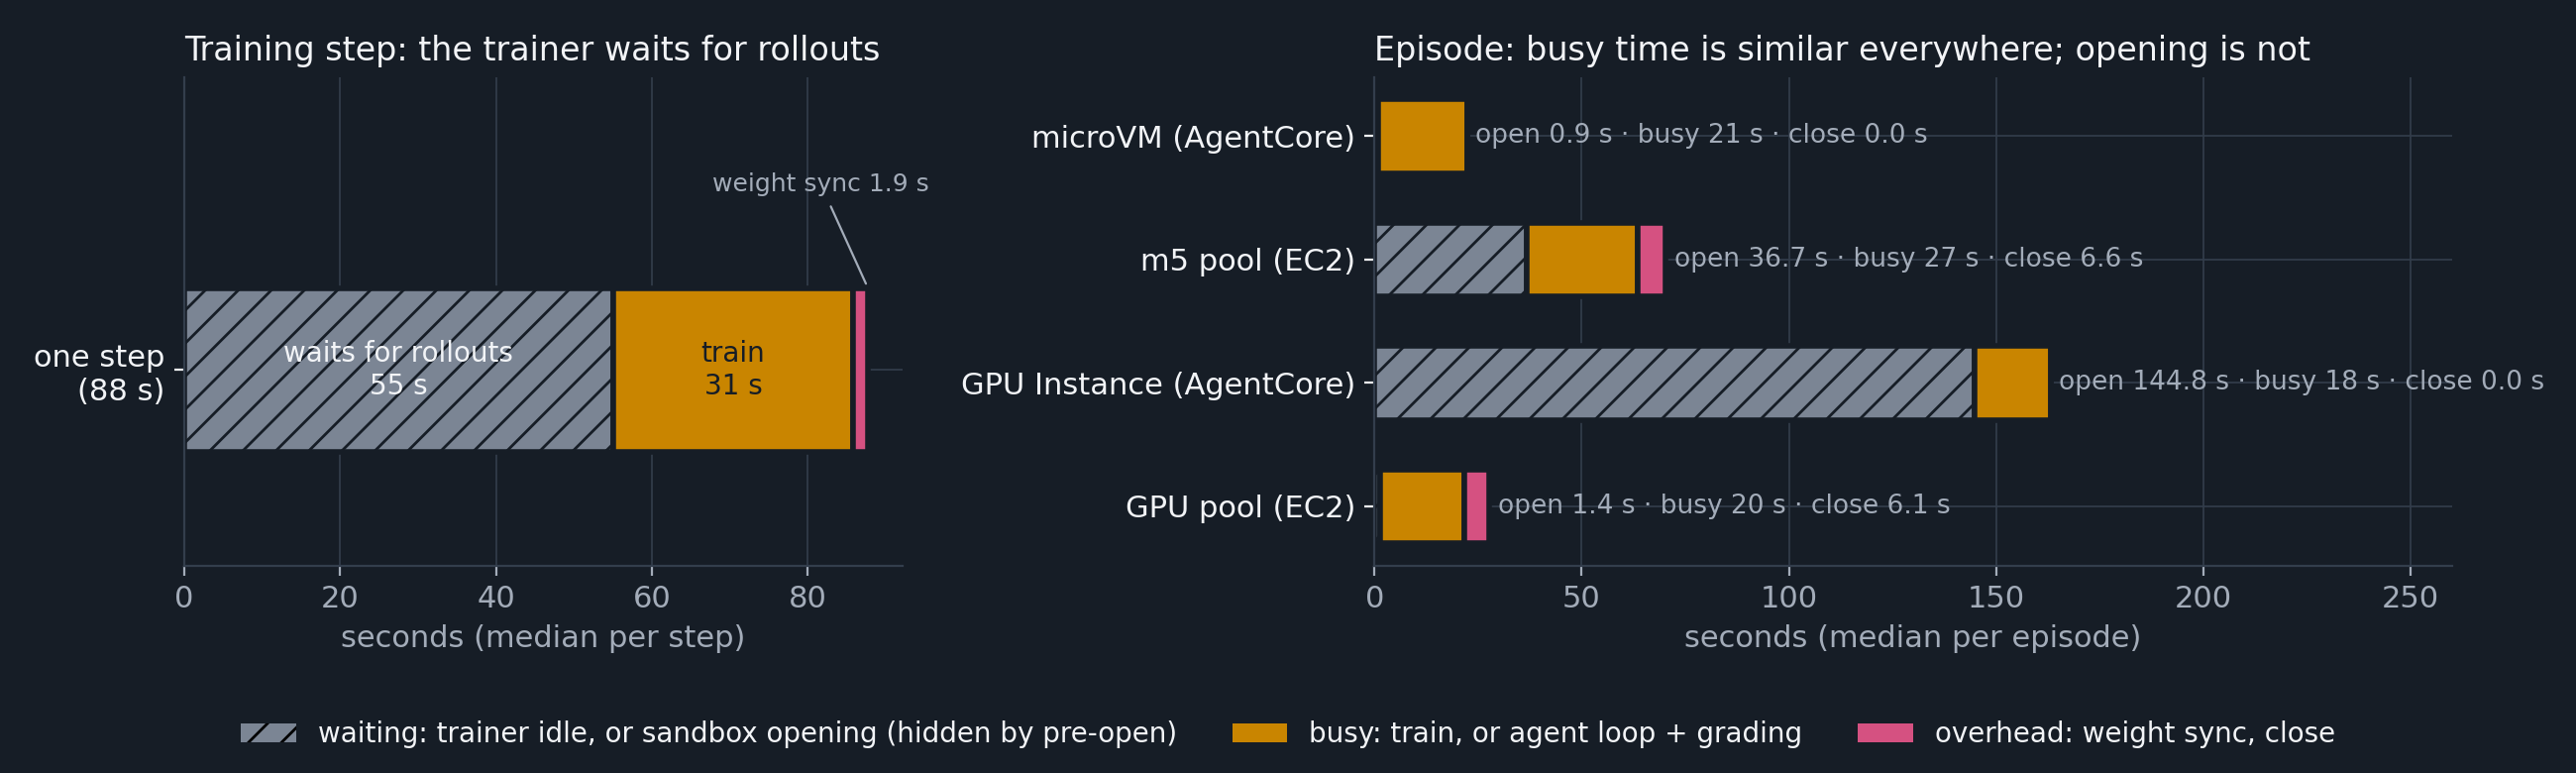
\includegraphics[width=0.97\linewidth]{fig_time.png}\par
\vspace{1mm}\raggedright
\begin{columns}[T]
\column{0.32\textwidth}
\begin{itemize}\footnotesize
\item \textbf{Step 88\,s}: 55\,s waiting for rollouts (model generation), 31\,s training, 1.9\,s weight sync.
\end{itemize}
\column{0.32\textwidth}
\begin{itemize}\footnotesize
\item \textbf{Episode work 18--27\,s} on every substrate: the substrate doesn't slow the agent.
\end{itemize}
\column{0.32\textwidth}
\begin{itemize}\footnotesize
\item \textbf{Opens differ 100$\times$} (0.9\,s to 145\,s); pre-open hides it: wait \hl{0\,s}.
\end{itemize}
\end{columns}
\par\vskip 0pt plus 1filll
\deep{``Time breakdown'', ``Sandbox latency''}
\end{frame}

%====================================================================
\begin{frame}{Key AI-infra results: 192 live sandboxes across four substrates}
\begin{columns}[T]
\column{0.62\textwidth}
\figcap{Full-epoch run: live sandbox sessions per substrate}
\centering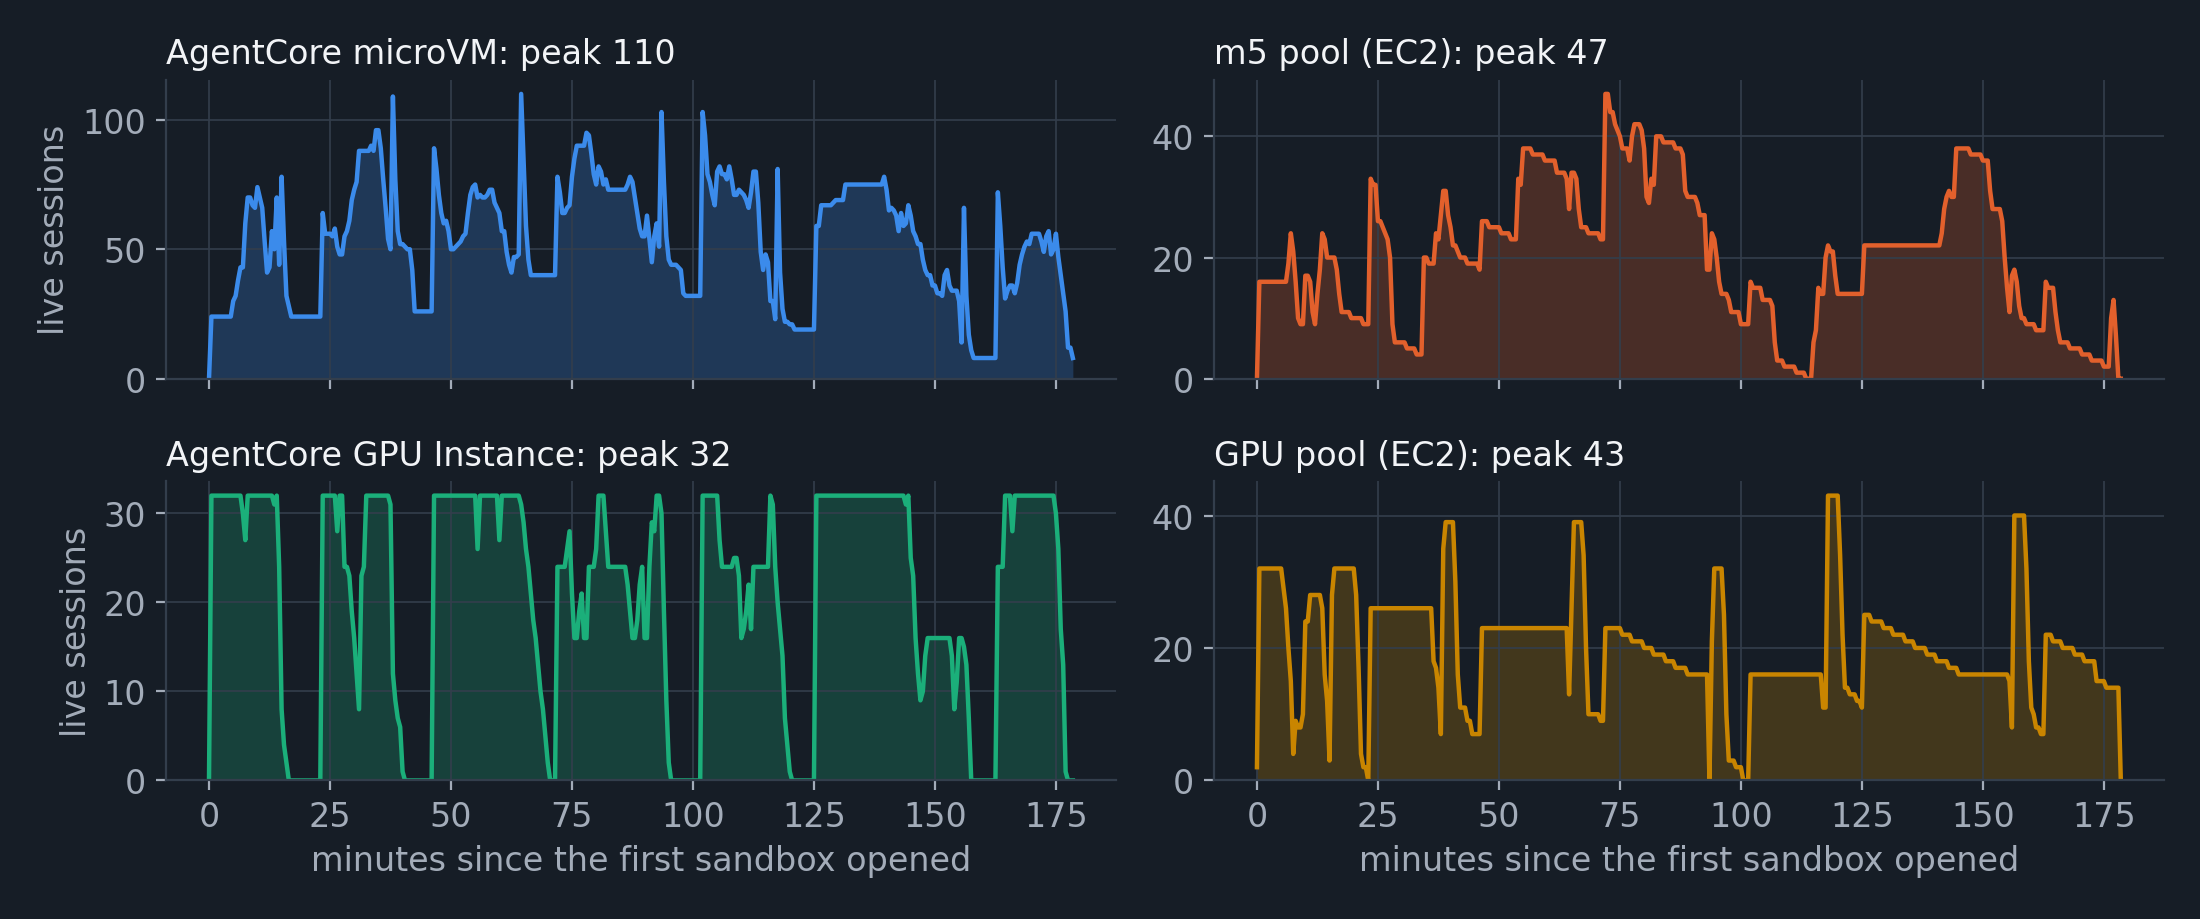
\includegraphics[width=\linewidth]{fig_concurrency.png}\par
\column{0.34\textwidth}
\begin{itemize}\footnotesize\setlength{\itemsep}{1.2mm}
\item \textbf{\hl{192} live sandboxes} at peak: 110 microVM, 47 m5, 32 AgentCore GPU, 43 GPU pool.
\item \textbf{32 episodes run at once}; the rest are pre-opened, ready for the next batches.
\item \textbf{Dips} are eval and checkpoint pauses.
\item \textbf{GPU capacity is the real limit}: g6 starved in all 4 AZs, so g5 did most of the work.
\end{itemize}
\end{columns}
\par\vskip 0pt plus 1filll
\deep{``Concurrency''}
\end{frame}

%====================================================================
\begin{frame}{Key AI-infra results: GPU reuse sets the cost; errors are rare}
\figcap{Full-epoch run (13 Oct): machine lifetimes and sessions served per machine}
\centering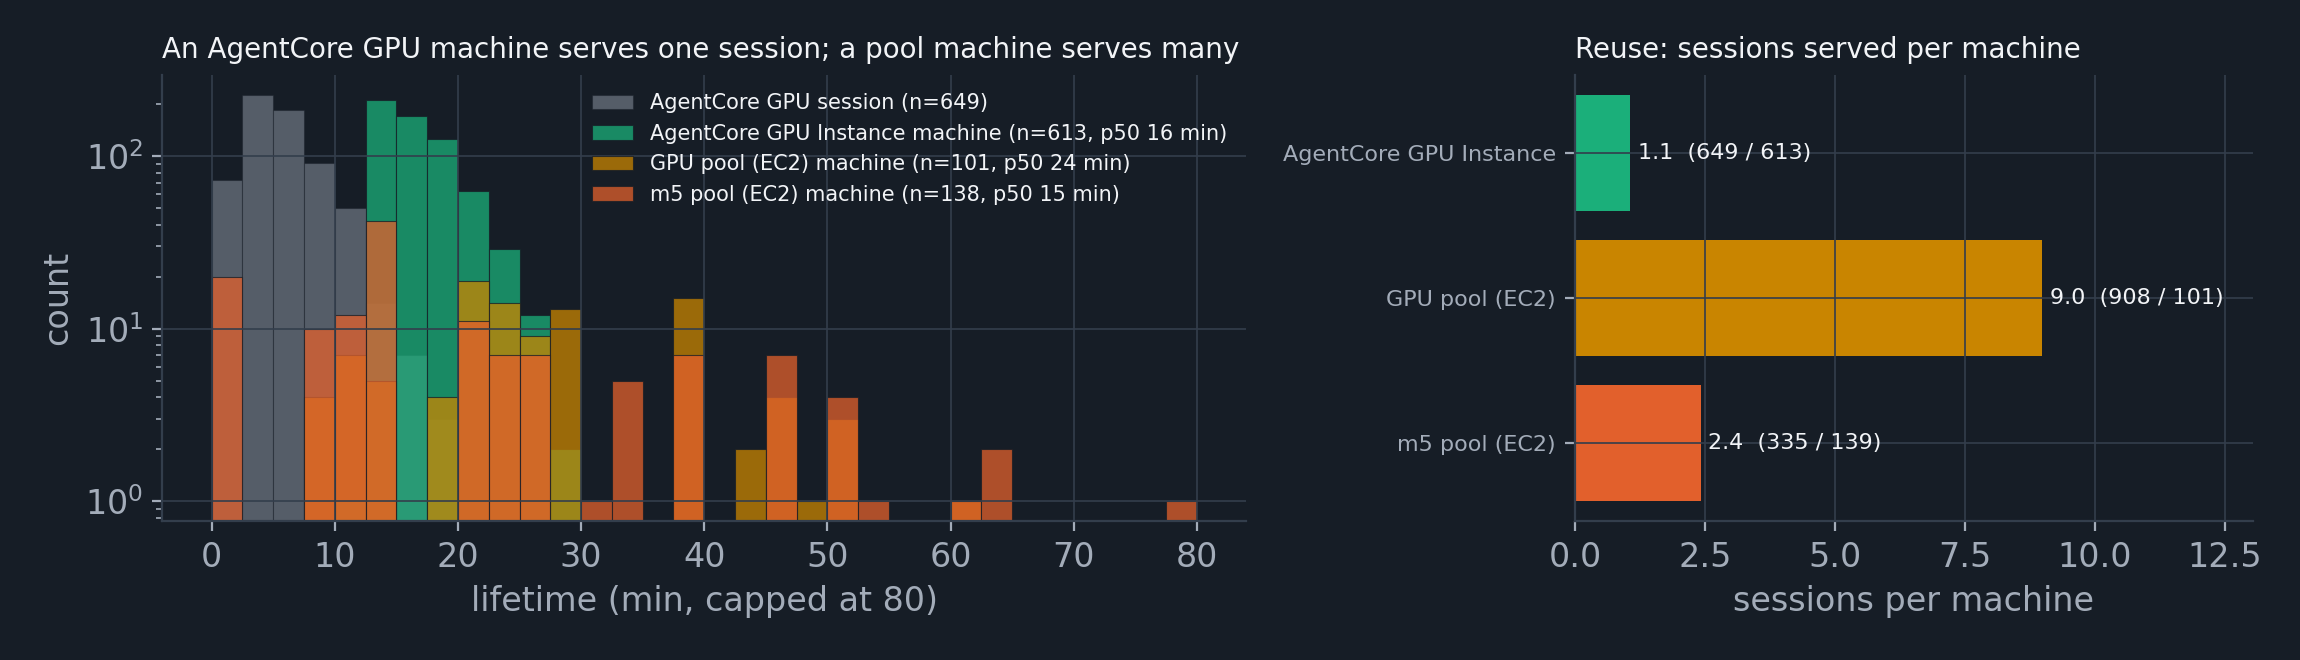
\includegraphics[width=0.97\linewidth]{fig_ev_ops.png}\par
\vspace{1mm}\raggedright
\begin{columns}[T]
\column{0.32\textwidth}
\begin{itemize}\footnotesize
\item \textbf{AgentCore GPU}: one machine per session; it lives \hl{16\,min} for a \hl{5.4\,min} session.
\end{itemize}
\column{0.32\textwidth}
\begin{itemize}\footnotesize
\item \textbf{EC2 pools reuse}: GPU pool \hl{908} episodes on 101 machines ($\sim$9 each); m5 2.4 each.
\end{itemize}
\column{0.32\textwidth}
\begin{itemize}\footnotesize
\item \textbf{\hl{0.34\,\%} infra errors} over all runs (69 in 20{,}154), mostly grading time-outs.
\end{itemize}
\end{columns}
\par\vskip 0pt plus 1filll
\deep{``Cost'', ``Reliability''}
\end{frame}

%====================================================================
\settag{Getting started}
\begin{frame}{Getting started}
\begin{columns}[T]
\column{0.48\textwidth}
{\normalsize\textbf{What you need}}
\begin{itemize}\small\setlength{\itemsep}{1.2mm}
\item An AWS account in a Region with AgentCore Runtime (built and tested in us-west-2).
\item A GPU host for training (here 8 GPUs), with the slime container.
\item Quotas: AgentCore Runtimes and sessions, EC2 vCPU; and \textbf{GPU capacity}, ideally reserved.
\item Your tasks in Terminal-Bench format: a Dockerfile, an instruction, hidden tests, a reference solution.
\end{itemize}
\column{0.48\textwidth}
{\normalsize\textbf{How it runs}}
\begin{enumerate}\small\setlength{\itemsep}{1.2mm}
\item Build the sandbox images and push them to Amazon ECR.
\item Register the Runtimes; every task's reference solution is checked where it will train.
\item Build the training data from the tasks that pass.
\item Train: a smoke run first ($\sim$20\,min), then full runs.
\item Clean up: one script removes what the run created.
\end{enumerate}
\vspace{1mm}
{\footnotesize Plan for the first image build: hours for a few hundred tasks.\par}
\end{columns}
\par\vskip 0pt plus 1filll
\plainen{bring tasks with hidden tests and a reference solution; the same pipeline routes, checks and trains them.}
\deep{``Prerequisites'', ``Run it end to end'', ``Bring your own tasks''}
\end{frame}

%====================================================================
{\bgframe{art/bg_close.png}
\begin{frame}[plain]
\vfill
{\fontsize{22}{26}\selectfont\bfseries\color{white}Thank you\par}
\vspace{3mm}
{\small\bfseries\color{white}Kaige Yang\par}
{\small\color{inkmuted}Senior Applied Scientist, AWS\par}
{\small\color{inkmuted}\href{mailto:kaigey@amazon.com}{kaigey@amazon.com}\par}
\vspace{2mm}
\vfill
\end{frame}}

\end{document}
